\documentclass{article}

\usepackage[
    examples=expex,
    font=lmodern,
    biblatex=false,
]{lingtex}
\usepackage{csquotes}
\usepackage{hologo}
\usepackage{graphicx,subfig}
\usepackage[heightadjust=all,valign=c]{floatrow}
\usepackage{fr-subfig}

\def\movesrc{\ensuremath{\circ}}
\def\lingtex{\texttt{lingtex}}

\title{Ling\TeX}
\author{Jackson Petty}
\date{\today}

\def\ipademo{f@"nEtIks}

\begin{document}
\maketitle

\noindent
Hello linguistics friends! This is some brief documentation for \texttt{lingtex}, a collection of \hologo{LaTeX} files that cover quite a lot of what you'll ever need to use \hologo{LaTeX} for in the NYU Linguistics department, and maybe beyond. I use this for my problem sets and term papers, and I hope you'll find it useful too.

\section{Installation \& Use} \label{sec:installation-use}

\lingtex\ is not an \enquote{official} \hologo{LaTeX} package, which means that it's not installed by default on your \hologo{LaTeX} distribution. Therefore, to use it, you'll need to copy the file(s) you need into whatever project you're working on.

If you're using Overleaf, I \emph{highly} recommend using the \enquote{Add From External URL} feature; this will allow you to import files directly from this GitHub repository into your Overleaf project \emph{and} you can update the files to a new version of I fix any bugs in the code. To do this, you'll need to copy the following URL:
$$
	\texttt{https://raw.githubusercontent.com/jopetty/lingtex/main/lingtex.sty}
$$
Next, click on the \enquote{File} button in the upper-left-hand corner of your Overleaf project (\ref{fig:a}). Click on the \enquote{From External URL} tab (\ref{fig:b}), and paste in the URL you just copied.  Then click the green \enquote{Create} button (\ref{fig:c}). If you ever need to update the file, click on it and then click on the green \enquote{Refresh} button (\ref{fig:d}).


\thisfloatsetup{subfloatrowsep=qquad}
\begin{figure}[!htbp]
	\captionsetup[subfigure]{justification=centering}
	\ffigbox{%
		\begin{subfloatrow}[3]%
			\ffigbox[\FBwidth]{\caption{Step 1}\label{fig:a}}{%
				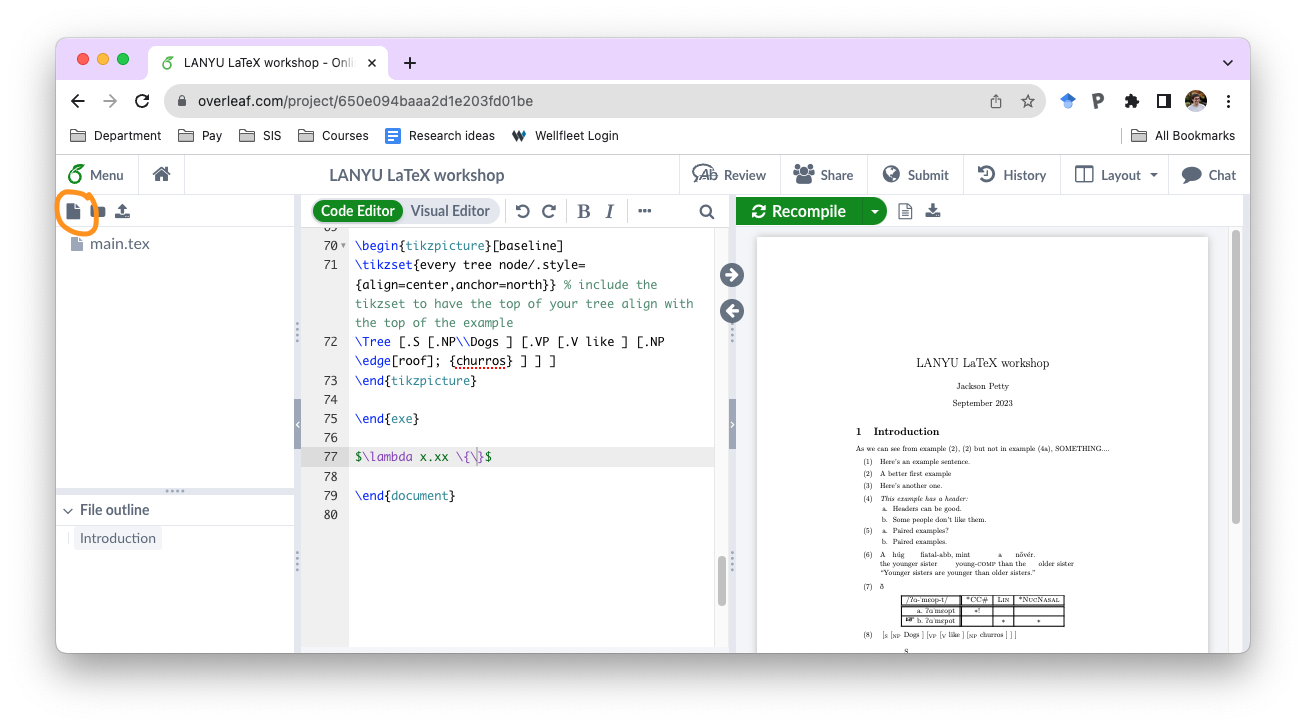
\includegraphics[width=0.455\textwidth]{images/step-1.png}}
			\ffigbox[\FBwidth]{\caption{Step 2}\label{fig:b}}{%
				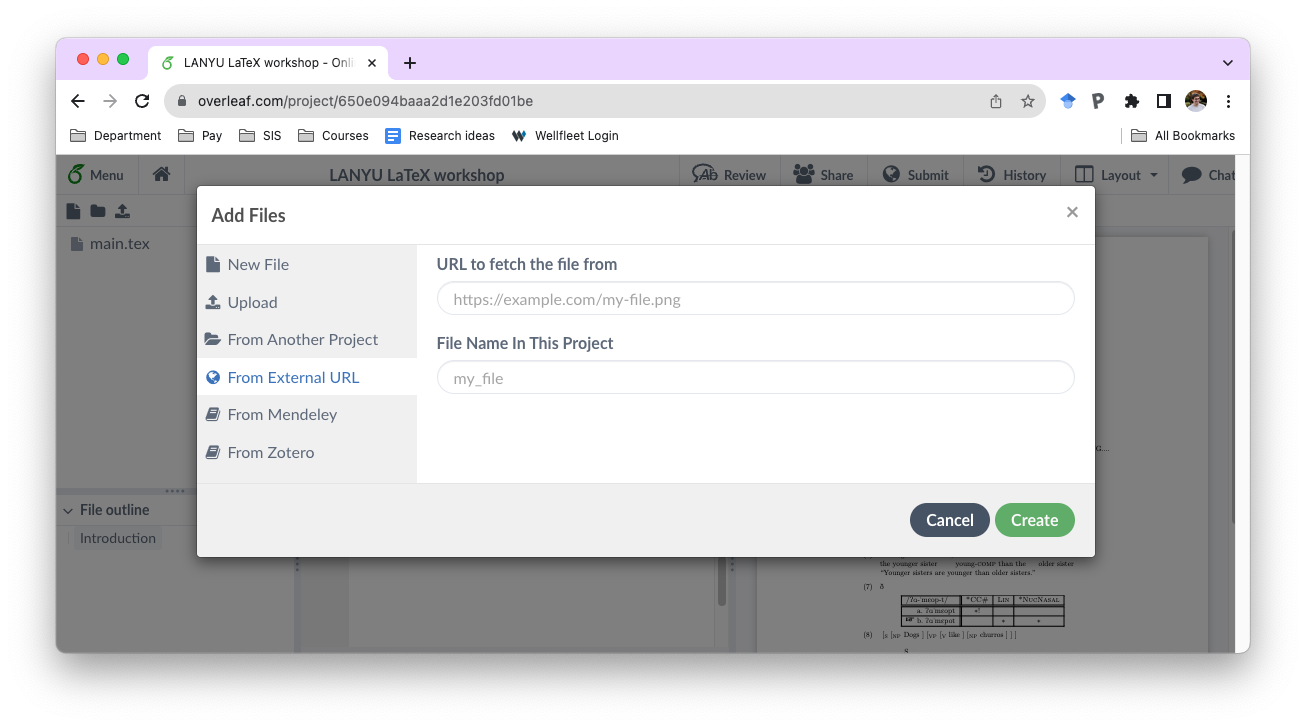
\includegraphics[width=0.45\textwidth]{images/step-2.png}}
		\end{subfloatrow}

		\begin{subfloatrow}
			\ffigbox[\FBwidth]{\caption{Step 3}\label{fig:c}}{%
				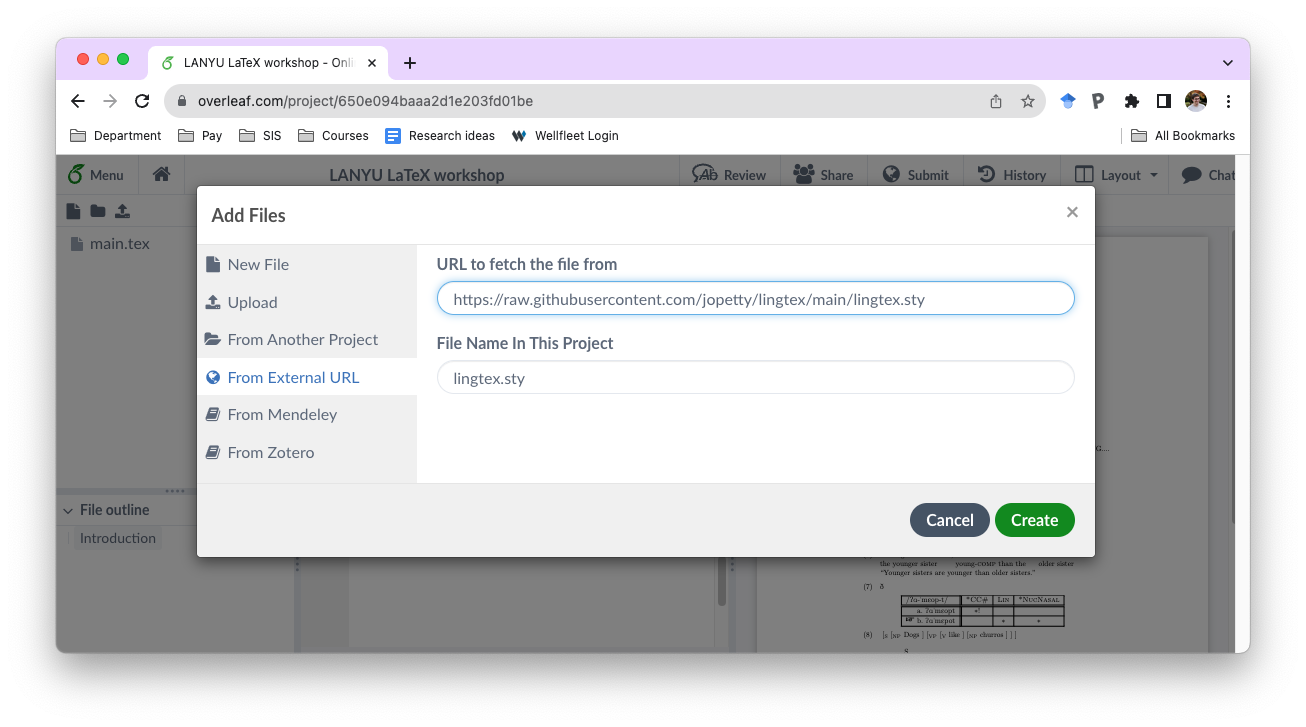
\includegraphics[width=0.45\textwidth]{images/step-3.png}}
			\ffigbox[\FBwidth]{\caption{Step 4}\label{fig:d}}{%
				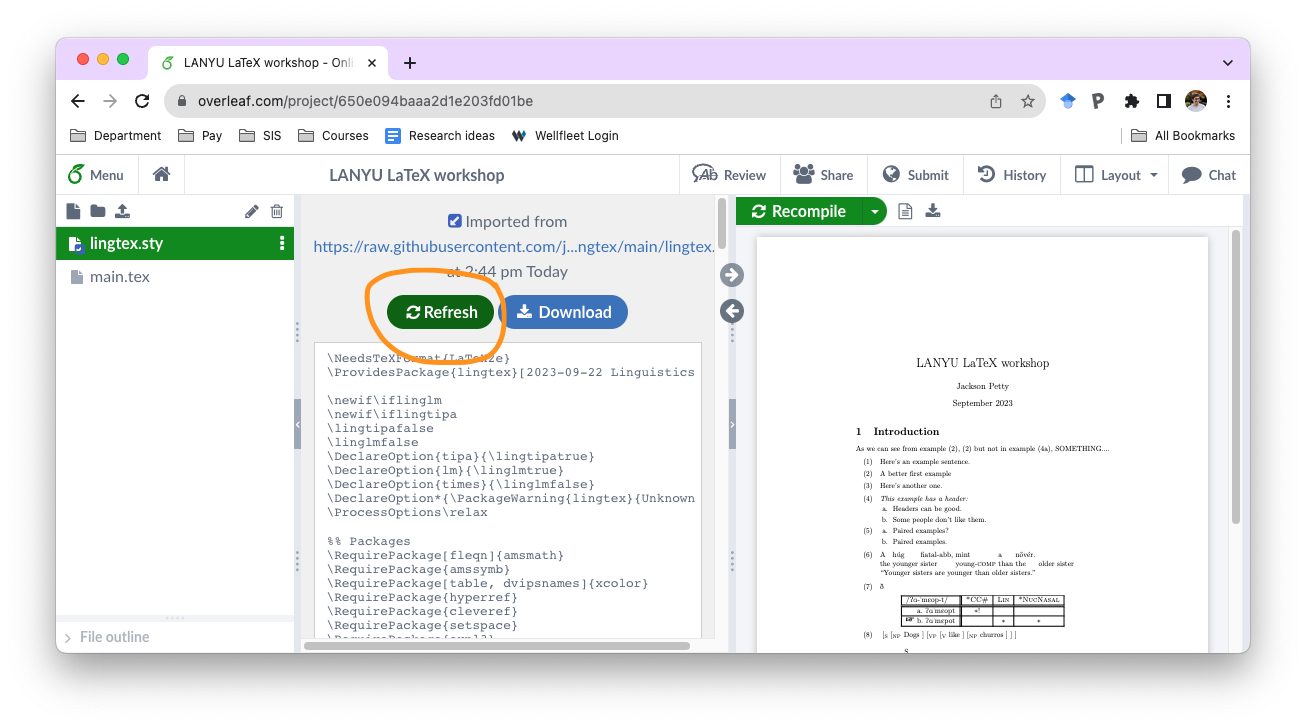
\includegraphics[width=0.45\textwidth]{images/step-4.png}}
		\end{subfloatrow}%
	}{}
\end{figure}

% \begin{figure}[htb!]
%     \ffigbox[\textwidth]
%       {
%         \begin{floatrow}
%         \ffigbox[\linewidth]
%           {
%           }
%           {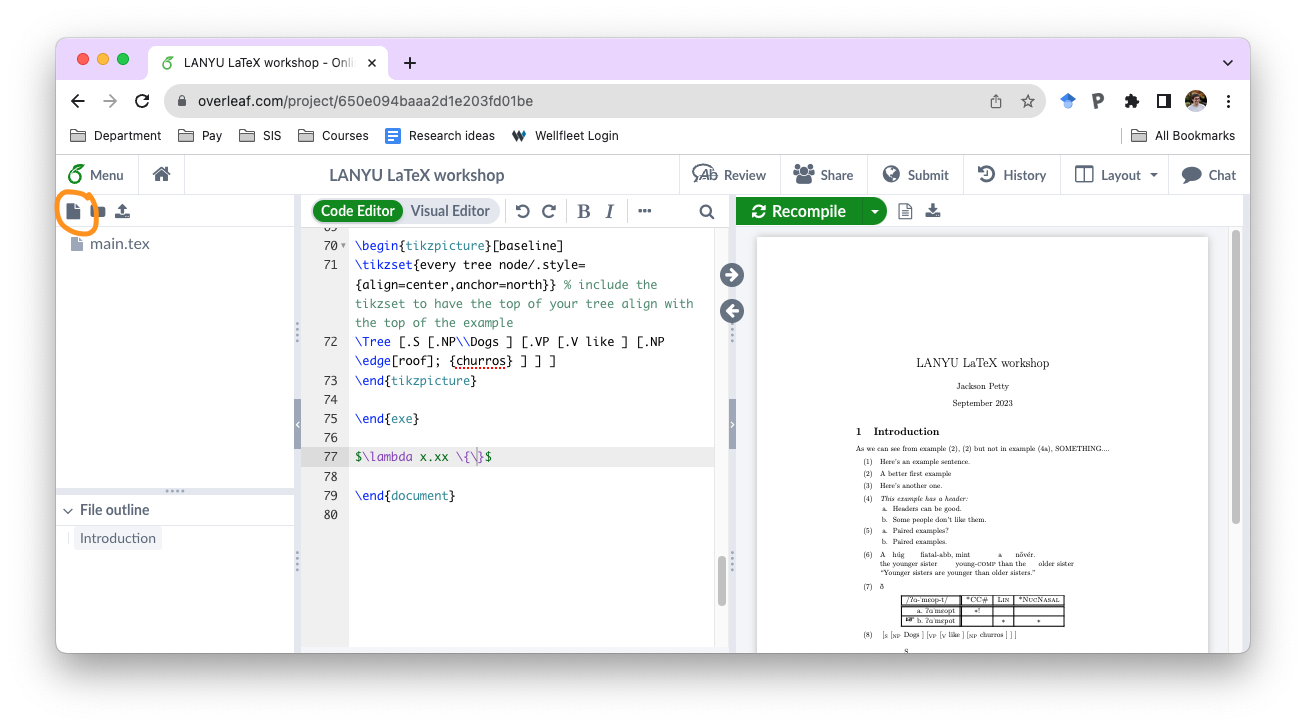
\includegraphics[width=\linewidth]{images/step-1.png}\caption{Step 1}\label{subfig:step-1}}
%         \ffigbox[\linewidth]
%           {
%           }
%           {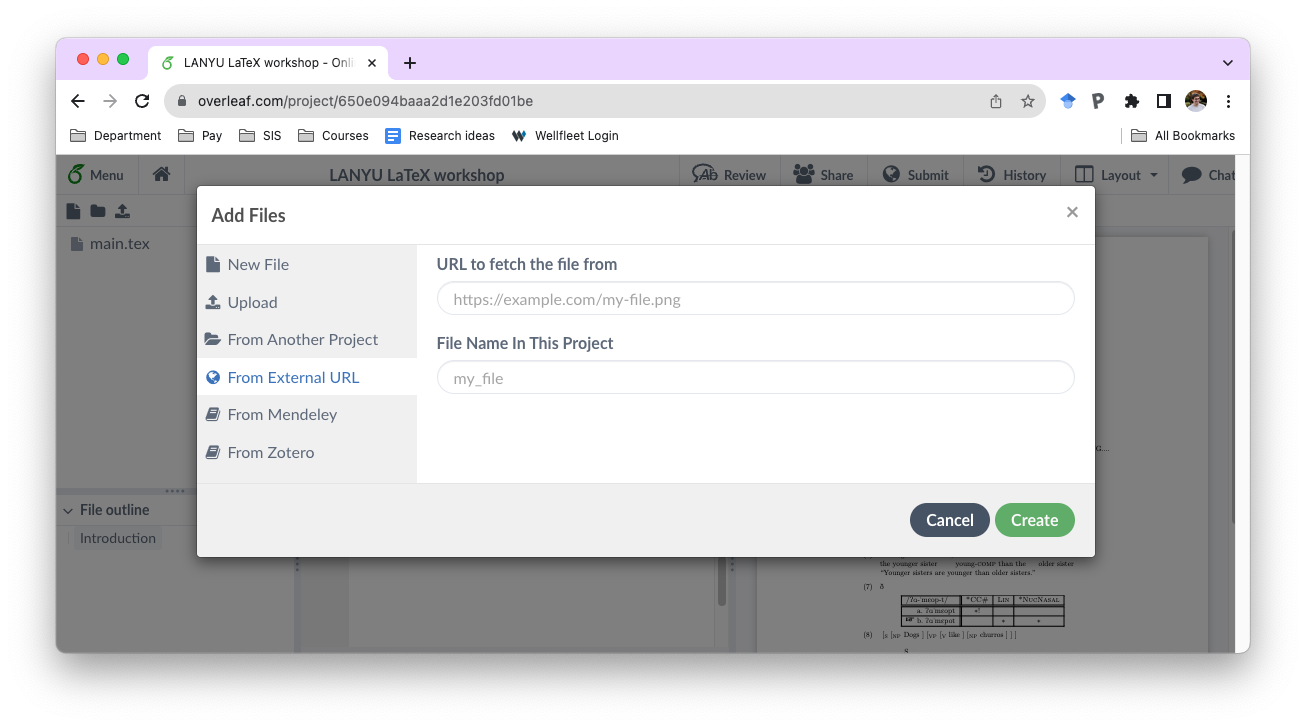
\includegraphics[width=\linewidth]{images/step-2.png}\caption{Step 2}\label{subfig:step-2}}
%         \end{floatrow}%
%         \newline
%         \begin{floatrow}
%             \ffigbox[\linewidth]
%               {
%               \label{subfig:step-3}}
%               {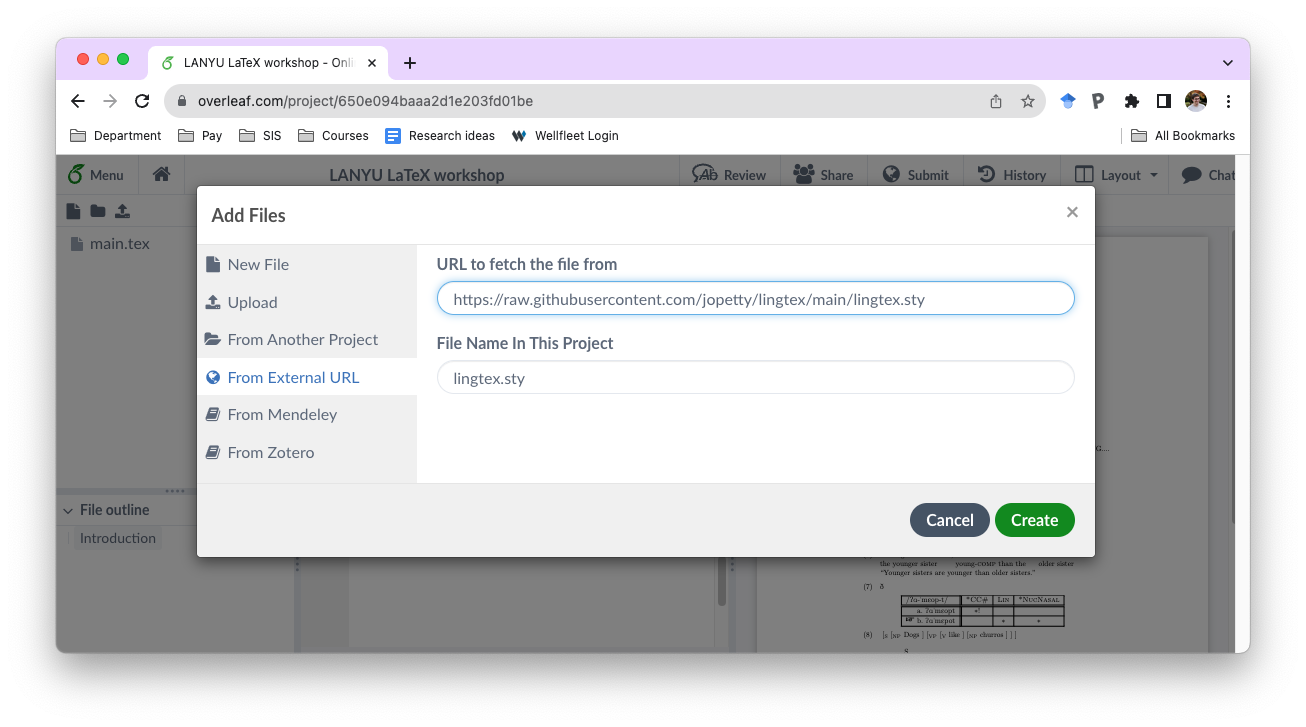
\includegraphics[width=\linewidth]{images/step-3.png}\caption{Step 3}}
%             \ffigbox[\linewidth]
%               {
%               \label{subfig:step-4}}
%               {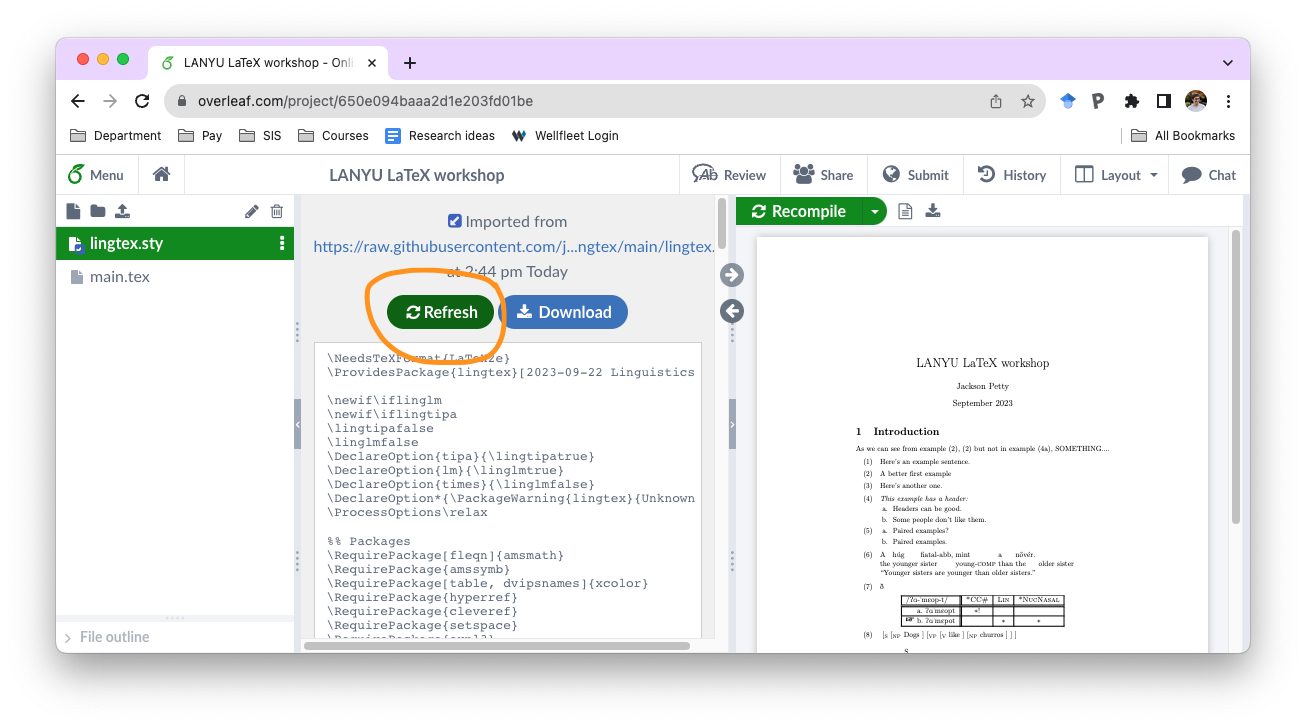
\includegraphics[width=\linewidth]{images/step-4.png}\caption{Step 4}}
%             \end{floatrow}%
%       }
%       {\label{fig:steps}}
% \end{figure}

\section{Linguistics Features} \label{sec:linguistics-features}

\lingtex\ provides a number of commands which are generally useful for linguistics:

\begin{itemize}
	\item \verb|\lex{}| for lexical items. This sets whatever argument you pass in in italics. For example, \verb|\lex{gato}| becomes \lex{gato}. It also allows you to provide an optional translation, which will be placed after in single quotes. For example, \verb|\lex[cat]{gato}| becomes \lex[cat]{gato}.
	\item \verb|\ipa{}| for IPA transcriptions. Internally, \lingtex\ defines a special command \verb|\ipafont| which you can set to an IPA font of your choice. We also load \verb|tipa| under the hood, so you can use any TIPA commands inside of \verb|\ipa{}|. For example, \verb|\ipa{f@"nEtIks}| becomes \ipa{f@"nEtIks}. We also define some additional commands which build on \verb|\ipa{}|:
	      \begin{itemize}
		      \item \verb|\allo{}| for allophones. This sets whatever argument you pass in in square brackets. For example, \verb|\allo{f@"nEtIks}| becomes \allo{f@"nEtIks}.
		      \item \verb|\phon{}| for phonemes. This sets whatever argument you pass in in slashes. For example, \verb|\phon{f@"nEtIks}| becomes \phon{f@"nEtIks}.
	      \end{itemize}
	\item \verb|\orth{}| for orthographic representations. This sets whatever argument you pass in in angle brackets. For example, \verb|\orth{cat}| becomes \orth{cat}. Note that this does \emph{not} use the \verb|\ipafont| under the hood, since orthographic representations are not written in IPA.
	\item \verb|\den{}| for semantic denotations. This sets whatever argument you pass in in double square brackets. For example, \verb|\den{cat}| becomes \den{cat}.
\end{itemize}

\section{Fonts} \label{sec:fonts}

\lingtex\ provides support for several common fonts choices. By default, documents are set in Times New Roman, since this is requested by most professors in the department. However, you can change this using the `font' option when loading the package. For example, to set the document in Computer Modern (the default `\hologo{LaTeX}' font) you can do the following:
\begin{verbatim}
    \usepackage[font=lmodern]{lingtex}
\end{verbatim}
Available options are:
\begin{itemize}
	\item \verb|times| for Times New Roman, uses the Doulos SIL font for IPA text;
	\item \verb|lmodern| for Computer Modern;
	\item \verb|libertinus| for Libertinus;
\end{itemize}

If you want to use a custom font, you can load it in the normal way (either by including a package for \hologo{pdfLaTeX} or by using \verb|fontspec| for \hologo{XeLaTeX} or \hologo{LuaLaTeX}). If you want to use a custom font for IPA text, you can set the \verb|\ipafont| command to the name of the font you want to use.

\section{Syntax} \label{sec:syntax}

\subsection{Examples} \label{ssec:examples}

\lingtex\ provides a way to auto-load various packages which provide support for numbered examples. By default, none of these will be loaded, since they can cause incompatibility with other code you may have already written. You can specify which package to load by passing the `examples' option to \lingtex\ when loading the package. For example, to use \texttt{expex} you would do the following:
\begin{verbatim}
    \usepackage[examples=expex]{lingtex}
\end{verbatim}
The supported options are:
\begin{itemize}
	\item \verb|expex|: Loads the \texttt{expex} package.
	\item \verb|gb4e|: Loads the \texttt{gb4e} package.
	\item \verb|linguex|: Loads the \texttt{linguex} package.
	\item \verb|covington|: Loads the \texttt{covington} package.
\end{itemize}
You can, of course, load any of these packages manually if you'd prefer, but \lingtex\ will also add some custom bug-fixes to make other package options play nicely with each other.

\subsection{Trees} \label{ssec:trees}

Similarly, \lingtex\ provides a way to auto-load various tree-drawing packages. By default, none are loaded, but you can specify which package to load with the \verb|trees| option. For example, to load \texttt{forest} you would do the following:
\begin{verbatim}
    \usepackage[trees=forest]{lingtex}
\end{verbatim}
The supported options are:
\begin{itemize}
	\item \verb|forest|: Loads the \texttt{forest} package.
	\item \verb|qtree|: Loads the \texttt{qtree} package.
	\item \verb|tikz-qtree|: Loads the \texttt{tikz-qtree} package.
	\item \verb|pstrees|: Loads the \texttt{pstrees} package.
\end{itemize}

\section{Phonology} \label{sec:phonology}

\subsection{OT Tableaux} \label{ssec:ot-tableaux}

Similarly, \lingtex\ provides a way to auto-load various tableaux packages. By default, none are loaded, but you can specify which package to load with the \verb|tableaux| option. For example, to load \texttt{ot-tableau} you would do the following:
\begin{verbatim}
    \usepackage[tableaux=ot-tableau]{lingtex}
\end{verbatim}
The supported options are:
\begin{itemize}
	\item \verb|ot-tableau|: Loads the \texttt{ot-tableau} package.
	\item \verb|OTtablx|: Loads the \texttt{OTtablx} package. \textbf{Warning:} This package uses \texttt{ps-tricks} under the hood, which is incompatible with \hologo{pdfLaTeX}. It won't throw an error if you try to use this option with \hologo{pdfLaTeX}, but it will display a warning.
\end{itemize}

\subsection{TIPA} \label{ssec:tipa}

By default, \lingtex\ will load \texttt{tipa} (if using \hologo{pdfLaTeX}) or \texttt{tipauni} (if using \hologo{XeLaTeX} or \hologo{LuaLaTeX}). This means that you can use TIPA syntax for entering IPA symbols with the \verb|\ipa{}| command.

If you don't want to use TIPA syntax, you can pass the \verb|tipa=false| option when loading the package.

\section{Bibliographies} \label{sec:bibliographies}

By default \lingtex\ will automatically load \texttt{biblatex} using the S\&P \verb|unified| style, created by the journal \emph{Semantics and Pragmatics}. This style should be acceptable for any term papers you'll have in the department. To use a bibliography, you will need to actually add the bib file as a resource, e.g., by adding
\begin{verbatim}
    \addbibresource{references.bib}
\end{verbatim}
to the preamble and then adding
\begin{verbatim}
    \printbibliography
\end{verbatim}
where you want the bibliography to appear.

If, however, you \emph{don't} want to use \texttt{biblatex}, you can pass the \verb|biblatex=false| option to \lingtex\ when loading the package. This will prevent \lingtex\ from loading \texttt{biblatex} in case you want to use a different bibliography package (like \texttt{natbib}) or if you to load \texttt{biblatex} manually with different options.

\end{document}